\documentclass{article}

% Packages
\usepackage{fancyhdr}
\usepackage{extramarks}
\usepackage{amsmath}
\usepackage{amsthm}
\usepackage{amsfonts}
\usepackage{tikz}
\usepackage[plain]{algorithm}
\usepackage{algpseudocode}
\usepackage{enumerate}
\usepackage{dsfont}
\usepackage{graphicx}
\usetikzlibrary{automata,positioning}

\graphicspath{ {./images} }

% Document Layout
\topmargin=-0.45in
\evensidemargin=0in
\oddsidemargin=0in
\textwidth=6.5in
\textheight=9.0in
\headsep=0.25in
\linespread{1.1}

% Page Style
\pagestyle{fancy}
\lhead{\hmwkAuthorName}
\chead{\hmwkClass:\ \hmwkTitle}
\rhead{Section \hmwkSection, \firstxmark}
\lfoot{\lastxmark}
\cfoot{\thepage}
\renewcommand\headrulewidth{0.4pt}
\renewcommand\footrulewidth{0.4pt}

% Paragraph Settings
\setlength\parindent{0pt}
\setlength{\parskip}{5pt}

% Section Management
\newcommand{\hmwkSection}{A} % Current section (A, B, or C) - update manually

% Problem Header Management
\newcommand{\enterProblemHeader}[1]{
  \nobreak\extramarks{}{Problem \arabic{#1} continued on next page\ldots}\nobreak{}
  \nobreak\extramarks{Problem \arabic{#1}}{Problem \arabic{#1} continued on next page\ldots}\nobreak{}
}

\newcommand{\exitProblemHeader}[1]{
  \nobreak\extramarks{Problem \arabic{#1}}{Problem \arabic{#1} continued on next page\ldots}\nobreak{}
  \stepcounter{#1}
  \nobreak\extramarks{Problem \arabic{#1}}{}\nobreak{}
}

% Counters
\setcounter{secnumdepth}{0}
\newcounter{partCounter}
\newcounter{homeworkProblemCounter}
\setcounter{homeworkProblemCounter}{1}
\nobreak\extramarks{Problem \arabic{homeworkProblemCounter}}{}\nobreak{}

% Homework Problem Environment
% Optional argument adjusts problem counter for non-sequential problems
\newenvironment{homeworkProblem}[1][-1]{
  \ifnum#1>0
    \setcounter{homeworkProblemCounter}{#1}
  \fi
  \section{Problem \arabic{homeworkProblemCounter}}
  \setcounter{partCounter}{1}
  \enterProblemHeader{homeworkProblemCounter}
}{
  \exitProblemHeader{homeworkProblemCounter}
}

% Assignment Details
\newcommand{\hmwkTitle}{Sheet\ \#1}
\newcommand{\hmwkDueDate}{October 24, 2025}
\newcommand{\hmwkClass}{C6.5 Theories of Deep Learning}
\newcommand{\hmwkClassInstructor}{Professor J. Tanner}
\newcommand{\hmwkAuthorName}{\textbf{Ray Tsai}}

% Title Page
\title{
  \vspace{2in}
  \textmd{\textbf{\hmwkClass:\ \hmwkTitle}}\\
  \normalsize\vspace{0.1in}\small{Due\ on\ \hmwkDueDate\ at 12:00pm}\\
  \vspace{0.1in}\large{\textit{\hmwkClassInstructor}} \\
  \vspace{3in}
}

\author{\hmwkAuthorName}
\date{}

% Part Command
\renewcommand{\part}[1]{\textbf{\large Part \Alph{partCounter}}\stepcounter{partCounter}\\}

% Mathematical Commands
% Algorithms
\newcommand{\alg}[1]{\textsc{\bfseries \footnotesize #1}}

% Calculus
\newcommand{\deriv}[1]{\frac{\mathrm{d}}{\mathrm{d}x} (#1)}
\newcommand{\pderiv}[2]{\frac{\partial}{\partial #1} (#2)}
\newcommand{\dx}{\mathrm{d}x}

% Probability and Statistics
\newcommand{\Var}{\mathrm{Var}}
\newcommand{\Cov}{\mathrm{Cov}}
\newcommand{\Bias}{\mathrm{Bias}}
\newcommand*{\prob}{\mathds{P}}
\newcommand*{\E}{\mathds{E}}

% Number Sets
\newcommand*{\Z}{\mathbb{Z}}
\newcommand*{\Q}{\mathbb{Q}}
\newcommand*{\R}{\mathbb{R}}
\newcommand*{\C}{\mathbb{C}}
\newcommand*{\N}{\mathbb{N}}

\begin{document}

\maketitle
\pagebreak

\begin{homeworkProblem}
  \textbf{Training Nets with Backpropagation and your first DNN classifier}

  \begin{enumerate}[(a)]
    \item Consider a standard feedforward network defined by $h^{(1)} = x$ and $h^{(j+1)} = \phi(W^{(j)}h^{(j)} + b^{(j)})$ for $j = 1,...,N-1$. Define the loss as the sum of squared errors, $\frac{1}{2m} \sum_{i=1}^m ||h^{(N)}(x_i) - y_i||^2$ over the $m$ data points, and derive the formulae used for `backpropagation' to update weights and biases when optimising the loss function using gradient descent.
    \begin{proof}
      Let $E_i = \frac{1}{2} ||h^{(N)}(x_i) - y_i||^2$, and let $L = \frac{1}{2m} \sum_{i=1}^m E_i$. Fix $i$. For $r = 1, \ldots, N - 1$, put $z^{(r + 1)} = W^{(r)}h^{(r)} + b^{(r)}$, and put $\delta^{(r)}_i = \frac{\partial E_i}{\partial z^{(r)}} = \nabla_{z^{(r)}} E_i$. By the chain rule,
      \[
        \delta^{(r)}_i = \frac{\partial E_i}{\partial z^{(r)}} = \frac{\partial E_i}{\partial h^{(r)}} \cdot \frac{\partial h^{(r)}}{\partial z^{(r)}} = \frac{\partial E_i}{\partial h^{(r)}} \cdot \phi'(z^{(r)}).
      \]
      When $r = N$, we have $\frac{\partial E_i}{\partial h^{(N)}} = h^{(N)}(x_i) - y_i$, so
      \[
        \delta^{(N)}_i = (h^{(N)}(x_i) - y_i) \cdot \phi'(z^{(N)}(x_i)).
      \]
      For $1 \leq r \leq N - 1$, we have the recursive formula
      \[
        \delta^{(r)}_i = \frac{\partial E_i}{\partial h^{(r)}} \cdot \frac{\partial h^{(r)}}{\partial z^{(r)}} = \frac{\partial E_i}{\partial z^{(r + 1)}} \cdot \frac{\partial z^{(r + 1)}}{\partial h^{(r)}} \cdot \frac{\partial h^{(r)}}{\partial z^{(r)}} = (W^{(r)})^T\delta^{(r + 1)}_i \cdot \phi'(z^{(r)}).
      \]
      Thus,
      \[
        \frac{\partial E_i}{\partial W^{(r)}} = \frac{\partial E_i}{\partial z^{(r + 1)}} \cdot \frac{\partial z^{(r + 1)}}{\partial W^{(r)}} = \delta^{(r + 1)}_i \cdot (h^{(r)}(x_i))^T,
      \]
      \[
        \frac{\partial E_i}{\partial b^{(r)}} = \frac{\partial E_i}{\partial z^{(r + 1)}} \cdot \frac{\partial z^{(r + 1)}}{\partial b^{(r)}} = \delta^{(r + 1)}_i.
      \]
      It now follows that
      \[
        \frac{\partial L}{\partial W^{(r)}} = \frac{1}{m} \sum_{i=1}^m \frac{\partial E_i}{\partial W^{(r)}} = \frac{1}{m} \sum_{i=1}^m \delta^{(r + 1)}_i \cdot (h^{(r)}(x_i))^T,
      \]
      \[
        \frac{\partial L}{\partial b^{(r)}} = \frac{1}{m} \sum_{i=1}^m \frac{\partial E_i}{\partial b^{(r)}} = \frac{1}{m} \sum_{i=1}^m \delta^{(r + 1)}_i.
      \]
    \end{proof}

    \item Consider a XOR problem with data points $x_i \in \{0,1\}^2$ where $(0,0)$ and $(1,1)$ are labeled 0, and $(1,0)$ and $(0,1)$ are labeled 1.
    \begin{enumerate}[i.]
      \item Can a linear classifier correctly classify these points? Sketch the domain and desired decision boundary to motivate your answer.
      \begin{proof}
        A linear classifer cannot correctly classify these points, as there does not exist a line that can separate the points $(0,0)$ and $(1,1)$ from the points $(1,0)$ and $(0,1)$.
      \end{proof}
      \item Train a single-hidden-layer network classifier with sigmoid activations from scratch (without help from Tensorflow or Pytorch) to solve XOR. In the attached notebook, calculate the required gradient updates and fill in the \texttt{NeuralNetwork.backprop()} function to train the network and visualise results. Note how the learnt decision boundary compares with expectations.
      \begin{proof}
        
      \end{proof}
    \end{enumerate}

    \item \textbf{The "Hello World" of supervised deep learning: MNIST digit classification.} 
    
    Now that you have trained a network from scratch yourself, you are unlikely to ever do this again. Deep learning libraries have developed high level APIs which make it very easy to quickly build and train models. The ability to use these APIs to quickly build and investigate small models is a very useful skill in (even theoretical) deep learning research, allowing you to run experiments and probe hypotheses.

    MNIST is a benchmark dataset of handwritten digits, that has approximately 70,000 example images from 10 classes. Each 2-dimensional image is of size '28 x 28', and belongs to one of the categories '0-9'. Fill in the code for the missing steps in the attached notebook to prepare the data, add layers to the model, compile the model with a loss function (which loss function will you use?), and then train, and finally evaluate, your model.

    % \url{https://colab.research.google.com/drive/1yLwyzhr2N6cAiSeJq6I0RpHy9vY5NBuH}
  \end{enumerate}
\end{homeworkProblem}

\newpage

% To change sections, use: \renewcommand{\hmwkSection}{B}
% Example: Uncomment the line below when you start Section B
\renewcommand{\hmwkSection}{B}

\begin{homeworkProblem}
  \textbf{Expressivity and depth}

  \begin{enumerate}[(a)]
    \item In Yarotsky (2016), it is proven that $f(x) = x^2$ on $[0,1]$ can be approximated with any error $\epsilon > 0$ by a ReLU network having depth and number of weights and computation units $O(\log(1/\epsilon))$. The proof relies on the following statement: 
    
    ``Let $f_m$ be the piece-wise linear interpolation of $f(x) = x^2$ with $2^m + 1$ uniformly distributed breakpoints $x_k = \frac{k}{2^m}, k=0,...,2^m$. The function $f_m$ approximates $f$ with the error $\epsilon_m = 2^{-2m-2}$ (in the $l_\infty$ norm).''
    
    Prove this statement.

    \begin{proof}
      Define $g_k = \frac{x_{k}^2 - x_{k - 1}^2}{x^k - x_{k - 1}} \cdot (x - x_{k - 1}) + x_{k - 1}^2$ for $k = 1, \ldots, 2^m$. Note that
      \[
        f_m(x) = \sum_{k = 1}^{2^m} g(x) \cdot \mathds{1}_{[x_k, x_{k + 1}]}(x).
      \]
      Since $f$ is increasing on $[0, 1]$, 
      \[
      \|f_m - f\|_\infty = \max_{x \in [0, 1]} |f_m(x) - f(x)| = \max_{k = 1, \ldots, 2^m} \max_{x \in [x_{k - 1}, x_k]} g_k(x) - x^2
      \]
      Put $E_k(x) = g_k(x) - x^2$ and we have
      \[
        E'_k(x) = \frac{x_{k}^2 - x_{k - 1}^2}{x^k - x_{k - 1}} - 2x.
      \]
      Thus, $E'_k(x)$ attains its maximum at $x = \frac{x_{k} + x_{k - 1}}{2}$. Substituting this into $E_k(x)$, we get
      \[
        \|f_m - f\|_\infty = \max_{k = 1, \ldots, 2^m} \frac{(x_{k} - x_{k - 1})^2}{4} = \frac{1}{4(2^m)^2} = 2^{-2m-2}.
      \]
    \end{proof}

    \item Recall from lectures that the `sawtooth' function can be created by iteratively composing the single-hidden-layer network $f(x) = \sigma(2\sigma(x) - 4\sigma(x-1/2))$, where $\sigma(x) = \max(x, 0)$. Can the same be achieved with a network of the same width and depth if hard-tanh activations are used instead of ReLU? If so, write down the corresponding function.
    \begin{proof}
      Let $\phi(x) = \max(0, \min(1, x))$ denote the hard sigmid function, and consider
      \[
        h(x) = \phi(2\phi(x) - 4\phi(x-1/2)) = \begin{cases}
          2x & \text{if } x \in [0, 1/2], \\
          2 - 2x & \text{if } x \in [1/2, 1], \\
          0 & \text{otherwise}.
        \end{cases}
      \]
      But then $h(x) = f(x)$. Thus the same result can be achieved with a network of the same width and depth by following the same iterative construction.
    \end{proof}

    \newpage

    \item Consider the $n$-alternating-point problem ($n$-ap problem). The dataset consists of $2^n$ uniformly spaced points within $[0, 1 - \frac{1}{2^n}]$ with alternating labels, i.e., pairs $((x_i, y_i))$ with $x_i = \frac{i}{2^n}$, and $y_i = 0$ when $i$ is even and $y_i = 1$ when $i$ is odd. How many layers does a width-2 ReLU network need to solve the $n$-ap problem? How wide would the layers need to be if there were only two layers?
    
    \begin{proof}
      Again, let $f_1(x) = \sigma(2\sigma(x) - 4\sigma(x-1/2))$ be the triangle function constructed using the ReLU function. Define
      \[
        f_n(x) = \sigma(2f_{n-1}(x) - 4f_{n-1}(x-1/2^n)).
      \]
      We proceed by induction to show that $f_n(x)$ is a piecewise linear function that oscillates between the points in the $n$-ap problem. The base case $n = 1$ is trivial. Suppose $n \geq 2$. By induction, $f_{n-1}(x)$ is a piecewise linear function that oscillates between the points in the $(n-1)$-ap problem. Note that $f_n(x)$ creates a triangle every time $f_{n - 1}(x)$ sweeps through $[0, 1]$, and that the triangles peak at $f^{-1}_{n - 1}(1/2)$. Since this happens twice for every triangle and $f_{n - 1}(x)$ has $2^{n - 1}$ triangles, $f_n(x)$ has $2^{n}$ triangles, each of which peaks at $x_i = i/2^n \in [0, 1 - 1/2^n]$ where $i$ is odd. This completes the induction. It now follows that $f_n(x)$ solves the $n$-ap problem, and that constructing it requires $n$ layers of width-2 ReLU network. Since $f_1$ has two layers and width 2, $f_n$ has $2n$ layers.

      Now suppose that we are restricted to using only two layers. That is, suppose
      \[
        f(x) = \phi\left(\sum_{j = 1}^m \alpha_j\phi(w_jx - b_j)\right)
      \]
      solves the $n$-ap problem. Note that each ReLU network in the sum allows us to alternate the slope of $f(x)$ once. Since we need to alternate the slop of $f(x)$ each time we enounter a new point, we require $2^n$ ReLU networks in the sum. Thus, $m = 2^n$ is the width required.
    \end{proof}

    \item Create an $n$-ap dataset for $n = 3$ and visualise the points by plotting. Then, implement and train a network of the minimum necessary depth (identified in the previous question) to solve the $n$-ap problem for $n = 8$ (refer to the code outline in the attached notebook). How well does it perform?
    
    \begin{proof}
      Terribly. Did I do something wrong or is shallow learning just ass? Like bro tf is ts??

      \begin{center}
        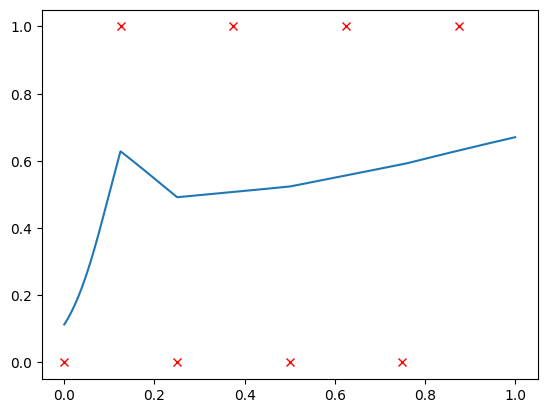
\includegraphics[width=0.5\textwidth]{2d.png}
      \end{center}
    \end{proof}

    \item Hardcode the weights that would solve the $n$-ap problem exactly (e.g., specify NN weights or compose the function $f(x) = \sigma(2\sigma(x) - 4\sigma(x-1/2))$ multiple times) and plot the result. Then, add small Gaussian noise ($\sigma = 0.1$) to the weights/coefficients. What happens to the function? What does this tell you about the loss function optimised to train the network in the previous question?
    
    \begin{proof}
      Adding some tiny noises to the weights completely ruins the function. It appears that the solution to this requires extreme precision on the weights. In particular, this shows that the model can easily get trapped in the local minima of the loss function, which would completely ruin the performance in this case.
      \begin{center}
        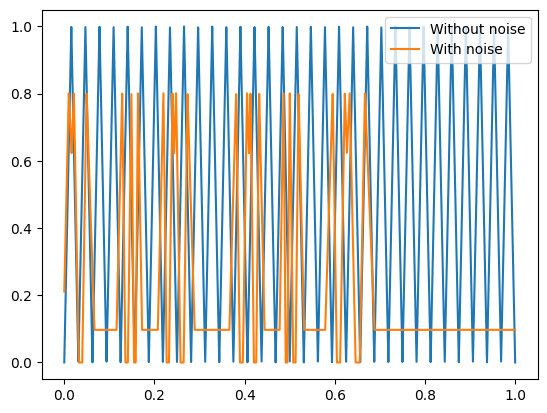
\includegraphics[width=0.5\textwidth]{2e.png}
      \end{center}
    \end{proof}

    \item Experiment with the associated Google Colab notebook code for approximating a one-dimensional piecewise smooth function. Vary the width and depth of the network. In other lectures, training options like batch-size and optimisation algorithms will be covered; the provided code defaults won't allow for high accuracy training. To contrast depth versus width with ReLU activations, compute the number of places where the slope changes in the generated function and consider the width needed to achieve the same approximation with a depth-2 network. Finally, try generating a two-dimensional piecewise smooth function and learn a network that approximates it.
  \end{enumerate}
\end{homeworkProblem}

\renewcommand{\hmwkSection}{C}

\end{document}